\chapter{Experimental implications}\label{chap:implications}

The Sommerfeld enhancement factor derived in Chapter \ref{chap:derivation} can greatly impact the interpretation of experimental limits set on the annihilation cross section by direct observation of gamma-ray production from the Galactic Centre, dwarf spheroidal galaxies and the Cosmic Microwave Background. In order to show this, I will consider a non-self-conjugate dark matter model and compare it to the limits coming from Fermi-LAT data.

\section{The Fermi-LAT limits}

Profumo et al. \cite{Profumo_2018} reviewed data coming from the H.E.S.S., Fermi-LAT and Planck collaborations to set upper bounds on the annihilation cross section in the hypothesis of self-conjugate dark matter. Fermi-LAT data concerns 15 dSphs, which are astronomical objects that, due to their very low velocity dispersion, are an interesting target to understand the implications of the Sommerfeld enhancement. The study assumes that dark matter preferentially annihilates into non-SM particles, like two short-lived dark mediators \(\phi \), that later decay into SM particles like quarks and leptons. This scenario is typically referred to as ``secluded dark matter''. For the sake of this research, I will only focus on the decay to \(4\tau \) leptons, so that the Fermi-LAT limit is the strongest one. This constrains the mass of the mediator to be
\begin{equation}\label{eq:mediator_mass}
	m_{\phi }  > 2 m_{\tau } 
\end{equation}
in order for the decay to be allowed. The Feynman diagram for this supposed decay is shown in Fig. \ref{fig:feynman}.

\begin{figure}[htbp]
	\centering
	\begin{tikzpicture}
		\begin{feynman}
			% Define the vertices
			\vertex (c) at (0, 0); % Central point

			% Incoming Dark Matter (DM) particles
			\vertex (dm1) [label=left:\(DM\)] at (-2, 1.5);
			\vertex (dm2) [label=left:\(\overline{DM}\)] at (-2, -1.5);

			% Intermediate vertices for V decay
			\vertex (v1) at (2, 1.5);
			\vertex (v2) at (2, -1.5);

			% Outgoing Standard Model (SM) particles
			\vertex (sm1) [label=right:\(\tau ^-\)] at (4, 2.25);
			\vertex (sm2) [label=right:\(\tau ^+\)] at (4, 0.75);
			\vertex (sm3) [label=right:\(\tau ^-\)] at (4, -0.75);
			\vertex (sm4) [label=right:\(\tau ^+\)] at (4, -2.25);

			% Draw the diagram edges (particles and propagators)
			\diagram* {
			(dm1) -- [fermion] (c),
			(dm2) -- [anti fermion] (c),
			(c) -- [photon, thick, edge label=\(\phi \)] (v1),
			(c) -- [photon, thick, edge label'=\(\phi \)] (v2),
			(v1) -- [fermion] (sm1),
			(v1) -- [anti fermion] (sm2),
			(v2) -- [fermion] (sm3),
			(v2) -- [anti fermion] (sm4),
			};
	
			\vertex[blob, fill=white, draw=black, postaction={pattern=north east lines}, minimum size=1cm] at (c) {}; % Hatched central vertex
		\end{feynman}
	\end{tikzpicture}
	\caption{The Feynman diagram for the secluded dark matter model we are investigating. Two dark matter particles annihilate into two mediators \(\phi \) that later decay to \(4\tau \) leptons.}
	\label{fig:feynman}
\end{figure}

In their study, Profumo et al. include results for different mass regimes, but I will only consider the ones for \(M_{DM} \gg M_{\phi } \) (in accordance with the hypothesis that the mediator mass is negligible). Moreover, the original Fermi-LAT limits must be weakened by a factor of \(2\), because dark matter is not its own antiparticle in the model I am considering.
% TODO: non sono convintissimo di questa frase
This effectively halves the chances of annihilation, allowing the cross section to double. In order to compare the limits to the theoretical predictions, I extracted the data from Figure 6 in \cite{Profumo_2018} by using a plot digitizer and I then interpolated them using a cubic spline, in order to plot them and to find the intersections with the theoretical values.
Both the original limits and the weakened limits are shown in Section \ref{sec:results} alongside the results in Fig. \ref{fig:comparison}, in a green and a black dashed line respectively.

\section{The impact of Sommerfeld enhancement}
The annihilation cross section of two dark matter particles into two mediators can be derived in quantum field theory and is independent of velocity. It can be expressed as
\begin{equation}
	\sigma v = \frac{\pi \alpha^2}{M_{DM}^2},
\end{equation}
% TODO: spiegare cosa è la dark matter relic abundance?
where \(\alpha\) is the strength of the interaction and \(M_{DM} \) is the mass of the dark matter particle. For non-self-conjugate dark matter, the value of the annihilation cross section that gives the correct dark matter relic abundance for \(M_{DM} > 10 \mathrm{GeV} \) is \(\langle \sigma v \rangle _{relic}  = 4.4 \times 10^{-26} \mathrm{cm^{-3} s^{-1}}\). Without Sommerfeld enhancement, this enforces a linear relation between the strength of the interaction and the mass of the dark matter particles:
\begin{equation}
	\alpha(M_{DM} ) = M_{DM} \sqrt{\frac{\langle \sigma v \rangle _{relic}}{\pi}}
\end{equation}

If Sommerfeld enhancement is relevant at the time of freeze-out, the situation is different, because the cross section must be corrected by multiplying by the Sommerfeld enhancement factor from Eq. \eqref{deriv:result}. The parameter \(\alpha \) must then satisfy the following equation:
\begin{equation}\label{eq:relic_Sommerfeld}
	\langle \sigma v \rangle _{relic} = \frac{2\pi \alpha ^3}{M_{DM} ^2} \frac{1 / v}{1- e^{-2\pi \frac{\alpha}{v}}},
\end{equation}
where \(v\) is the relative velocity between the two dark matter particles, which at freeze-out satisfies
\begin{equation}
	\left \langle \frac{1}{v} \right \rangle \simeq 4
\end{equation}
More precisely, one should compute a thermal average of the Sommerfeld enhancement factor and use that in Eq. \eqref{eq:relic_Sommerfeld}, but at these velocities the difference between an averaged enhancement factor and the same factor calculated at \(v= \langle v \rangle \) is almost non-existent. Equation \eqref{eq:relic_Sommerfeld} does not have an analytic solution and must therefore be solved with numerical tools. Fig. \ref{fig:alpha} compares \(\alpha (M_{DM} )\) in the two cases and shows that the difference becomes noticeable for masses around \(1 \mathrm{TeV} \).

\begin{figure}[htbp]
	\centering
	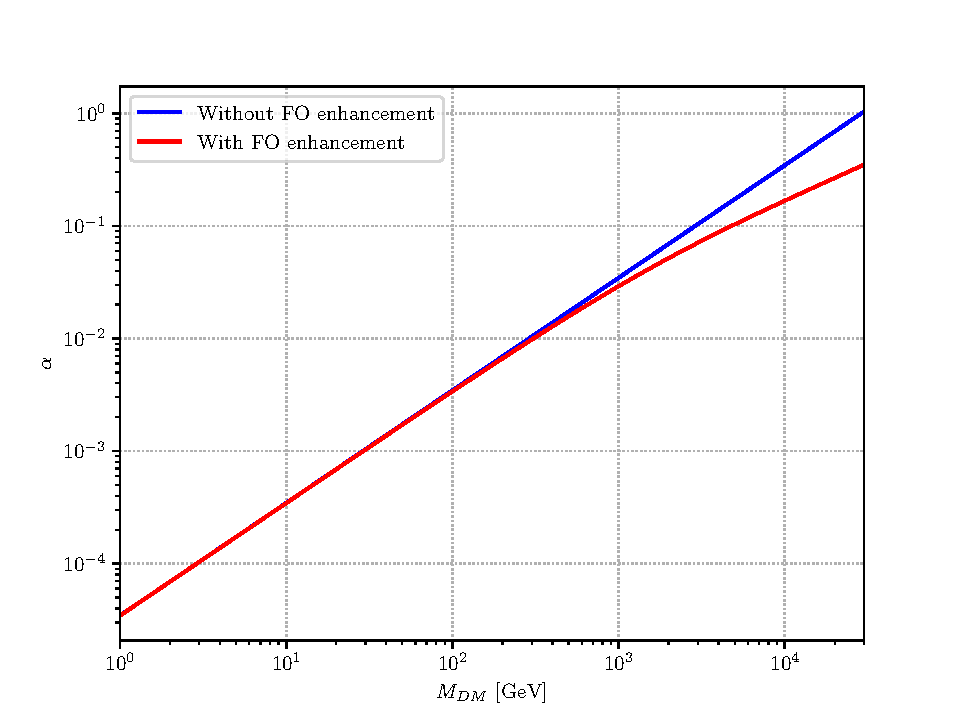
\includegraphics[width=0.9\textwidth]{alpha.pdf}
	\caption{Comparison between the \(\alpha (M_{DM} )\) relations with and without Sommerfeld enhancement at freeze-out, in red and blue respectively. \(\langle 1 / v \rangle \simeq 4 \) at freeze-out.}
	\label{fig:alpha}
\end{figure}

We can now use the corrected \(\alpha (M_{DM} )\) dependence to visualize the Sommerfeld enhancement factor (Fig. \ref{fig:enhancement_factor}) as a function of \(M_{DM} \) and of the relative velocity in units of \(c\) and confirm that it has indeed a huge impact on the cross section (\(2-4\) orders of magnitude) at low velocities like those found in dSphs.

\begin{figure}[htbp]
	\centering
	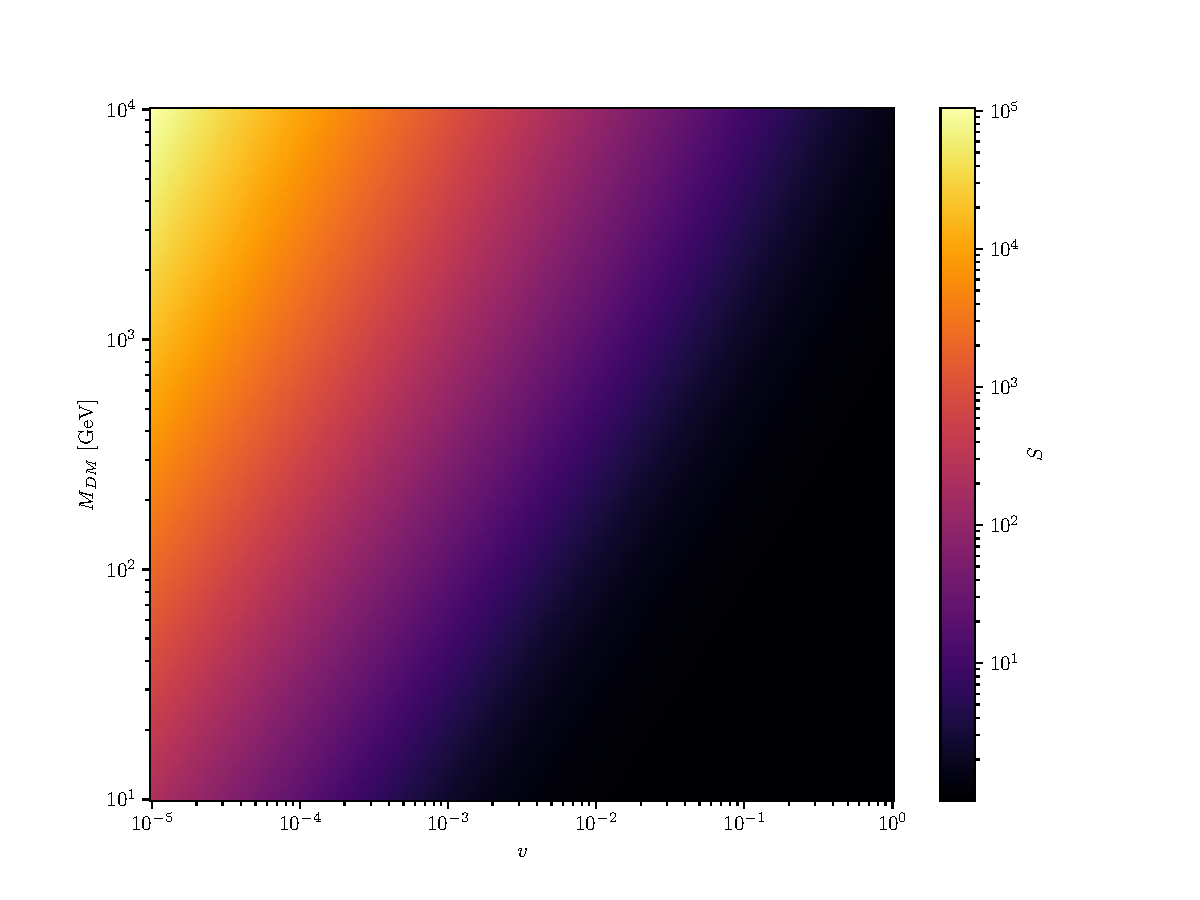
\includegraphics[width=0.9\textwidth]{enhancement_factor_color.pdf}
	\caption{The Sommerfeld enhancement factor for the range of masses \(M_{DM} \) relevant for the Fermi limits. The velocity axis ranges from the typical velocities in dSphs (\(\sim 10^{-5} \)) to the speed of light. One can notice that the effect is greater at lower velocities, like those in dSphs, and at higher masses.}
	\label{fig:enhancement_factor}
\end{figure}

The predicted cross section with the corrected \(\alpha (M_{DM} )\) is
\begin{equation}\label{eq:sigma_enhanced}
	\langle \sigma v \rangle (M_{DM} )= \frac{\pi \alpha (M_{DM} )^2}{M_{DM} ^2} \left \langle S \right \rangle(M_{DM} ),
\end{equation}
where the angle brackets indicate a thermal average over the Maxwell-Boltzmann distribution for the relative velocity. Here, averaging over the distribution is more important compared to the case at freeze-out and \(\langle S \rangle \neq S|_{v= \langle v \rangle }\). The typical line-of-sight velocity dispersion in dSphs is \(10 \mathrm{km / s} \) \cite{Walker_2013, Arkani_2009}. To find the three-dimensional velocity dispersion, we can assume that velocity is isotropic, thus giving a single-particle velocity dispersion of \(\beta = 10 \sqrt{3} \mathrm{km / s} \). One can show that the relative velocity dispersion \(\beta_{rel} \) is related to the single-particle velocity dispersion \(\beta \) by \(\beta _{rel} = \sqrt{2} \beta \) (see Appendix \ref{appendix:onebody} and \cite{Ferrer_2013}), hence the relative velocity PDF is
\begin{equation}
	P(v ) = \left( \frac{1}{4\pi } \right)^\frac{1}{2} \frac{v ^2}{\beta ^3} \exp \left( -\frac{v ^2}{4 \beta ^2} \right),
\end{equation}
The averaged Sommerfeld enhancement factor, which I computed numerically, is therefore
\begin{equation}
	\langle S \rangle (M_{DM} ) = \int\limits_0^{+ \infty } P(v ) S(M_{DM}, v ) \mathrm{d} v
\end{equation}


\section{Results}\label{sec:results}
In the simple case of no Sommerfeld enhancement and therefore of a linear \(\alpha (M_{DM} )\), the predicted cross section is
\begin{equation}
	\langle \sigma v \rangle = \langle \sigma v \rangle _{relic}
\end{equation}
for any value of \(M_{DM} \). Since the Fermi-LAT limits are upper bounds on the cross section, we want the predicted cross section to be lower than the limits and this constrains the dark matter mass to be
\begin{equation}\label{eq:result_simple}
	M_{DM} \gtrsim 80 \mathrm{GeV}, 
\end{equation}
which is where the blue horizontal line of \(\langle \sigma v \rangle _{relic} \) and the weakened interpolated Fermi-LAT limits meet in Fig. \ref{fig:comparison}.

The same reasoning can be applied to the enhanced cross section from Eq. \ref{eq:sigma_enhanced}, which is shown as a solid red line. Following the same reasoning as before, we find that
\begin{equation}\label{eq:result_enhanced}
	M_{DM} \gtrsim 9.9 \mathrm{TeV}
\end{equation}
in the case with Sommerfeld enhancement. Figure \ref{fig:comparison} summarizes these findings and clearly shows where the constraints come from. We conclude that the presence of Sommerfeld enhancement can impact by orders of magnitude the constraints we put on the dark matter mass, as can be clearly seen by comparing Eq. \ref{eq:result_simple} and Eq. \ref{eq:result_enhanced}. This has deep experimental implications, because it changes the way experiments have to look for this dark matter.

\begin{figure}[!ht]
	\centering
	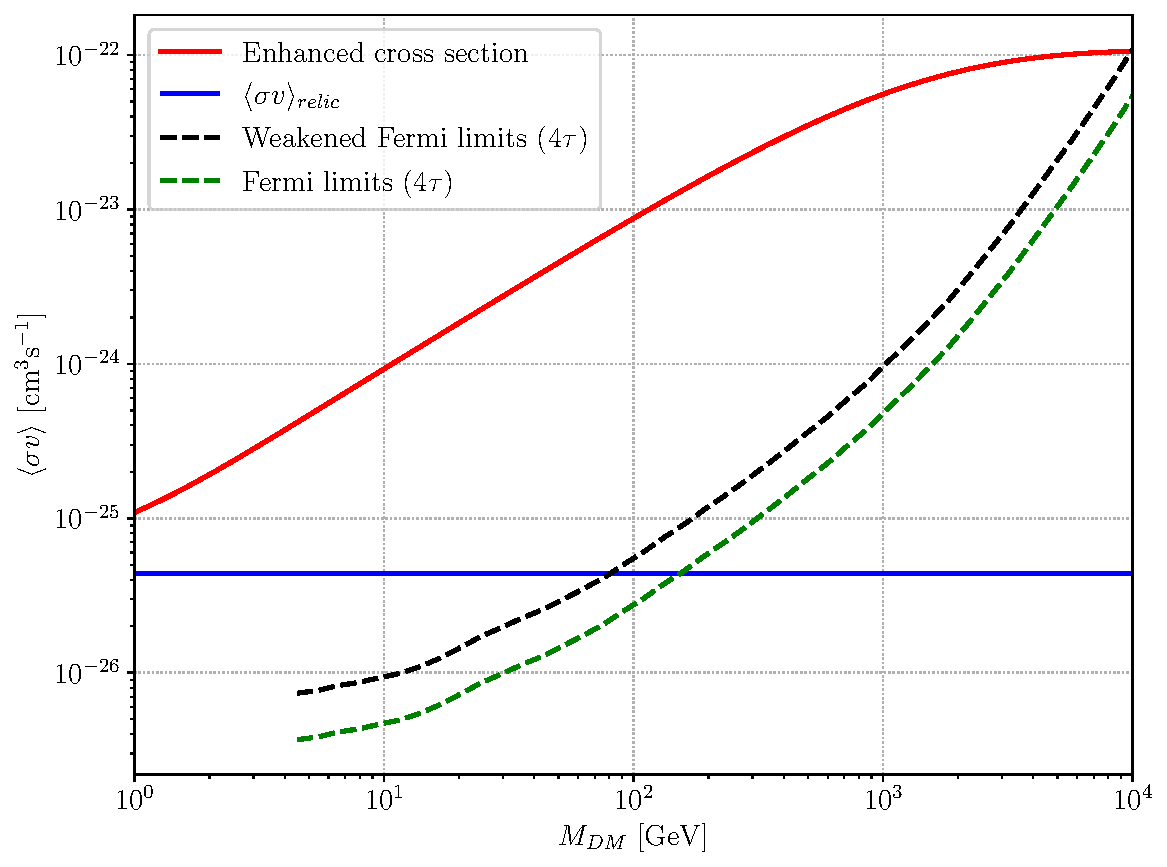
\includegraphics[width=0.9\textwidth]{comparison.pdf}
	\caption{Comparison between theoretical prediction and experimental limits set by Fermi-LAT data.}
	\label{fig:comparison}
\end{figure}

\section{Validity of the Coulomb approximation}

We must now check whether using the Coulomb approximation was appropriate in this case. As stated in Eq. \eqref{eq:Coulomb_approx}, the Coulomb approximation is valid if
\begin{equation}
	\frac{M_{DM} v}{2 m_{\phi } } \geq 1,
\end{equation}
As mentioned in Eq. \eqref{eq:mediator_mass}, \(m_{\phi } > 2 m_{\tau } \), and we have just found \(M_{DM} \gtrsim 9.9 \mathrm{TeV} \) in Eq. \eqref{eq:result_enhanced}. For the relative velocity \(v\), I am using its average value \(\langle v \rangle = 4 \beta /\sqrt{\pi } \) where \(\beta = 10 \sqrt{3}  \mathrm{km / s} \) as before. Calculating this ratio with the minimum allowed masses yields \(\sim 0.18\), meaning that the Coulomb approximation is actually not a good approximation in this case. Still, it gives us a good idea of the great effect that the Sommerfeld enhancement can have on constraints that we put on dark matter mass.

Since the Coulomb approximation is not valid in this case, one should resort back to a Yukawa potential that does account for the mediator mass. In this case, the Schrödinger equation does not have an analytic solution and must be solved numerically. Alternatively, the Yukawa potential can be approximated by the Hulthen potential, which gives an equation that does have an analytic solution. The main qualitative difference in this case is that the Sommerfeld effect saturates at low velocities: the supposed dark force has a finite range, and this limits how big the enhancement can get. This will change the precise constraints on the mass, but the Sommerfeld enhancement will still be around the same order of magnitude \cite{Arkani_2009}.